\section{Lighting}

\begin{figure}[H]
  \centering
  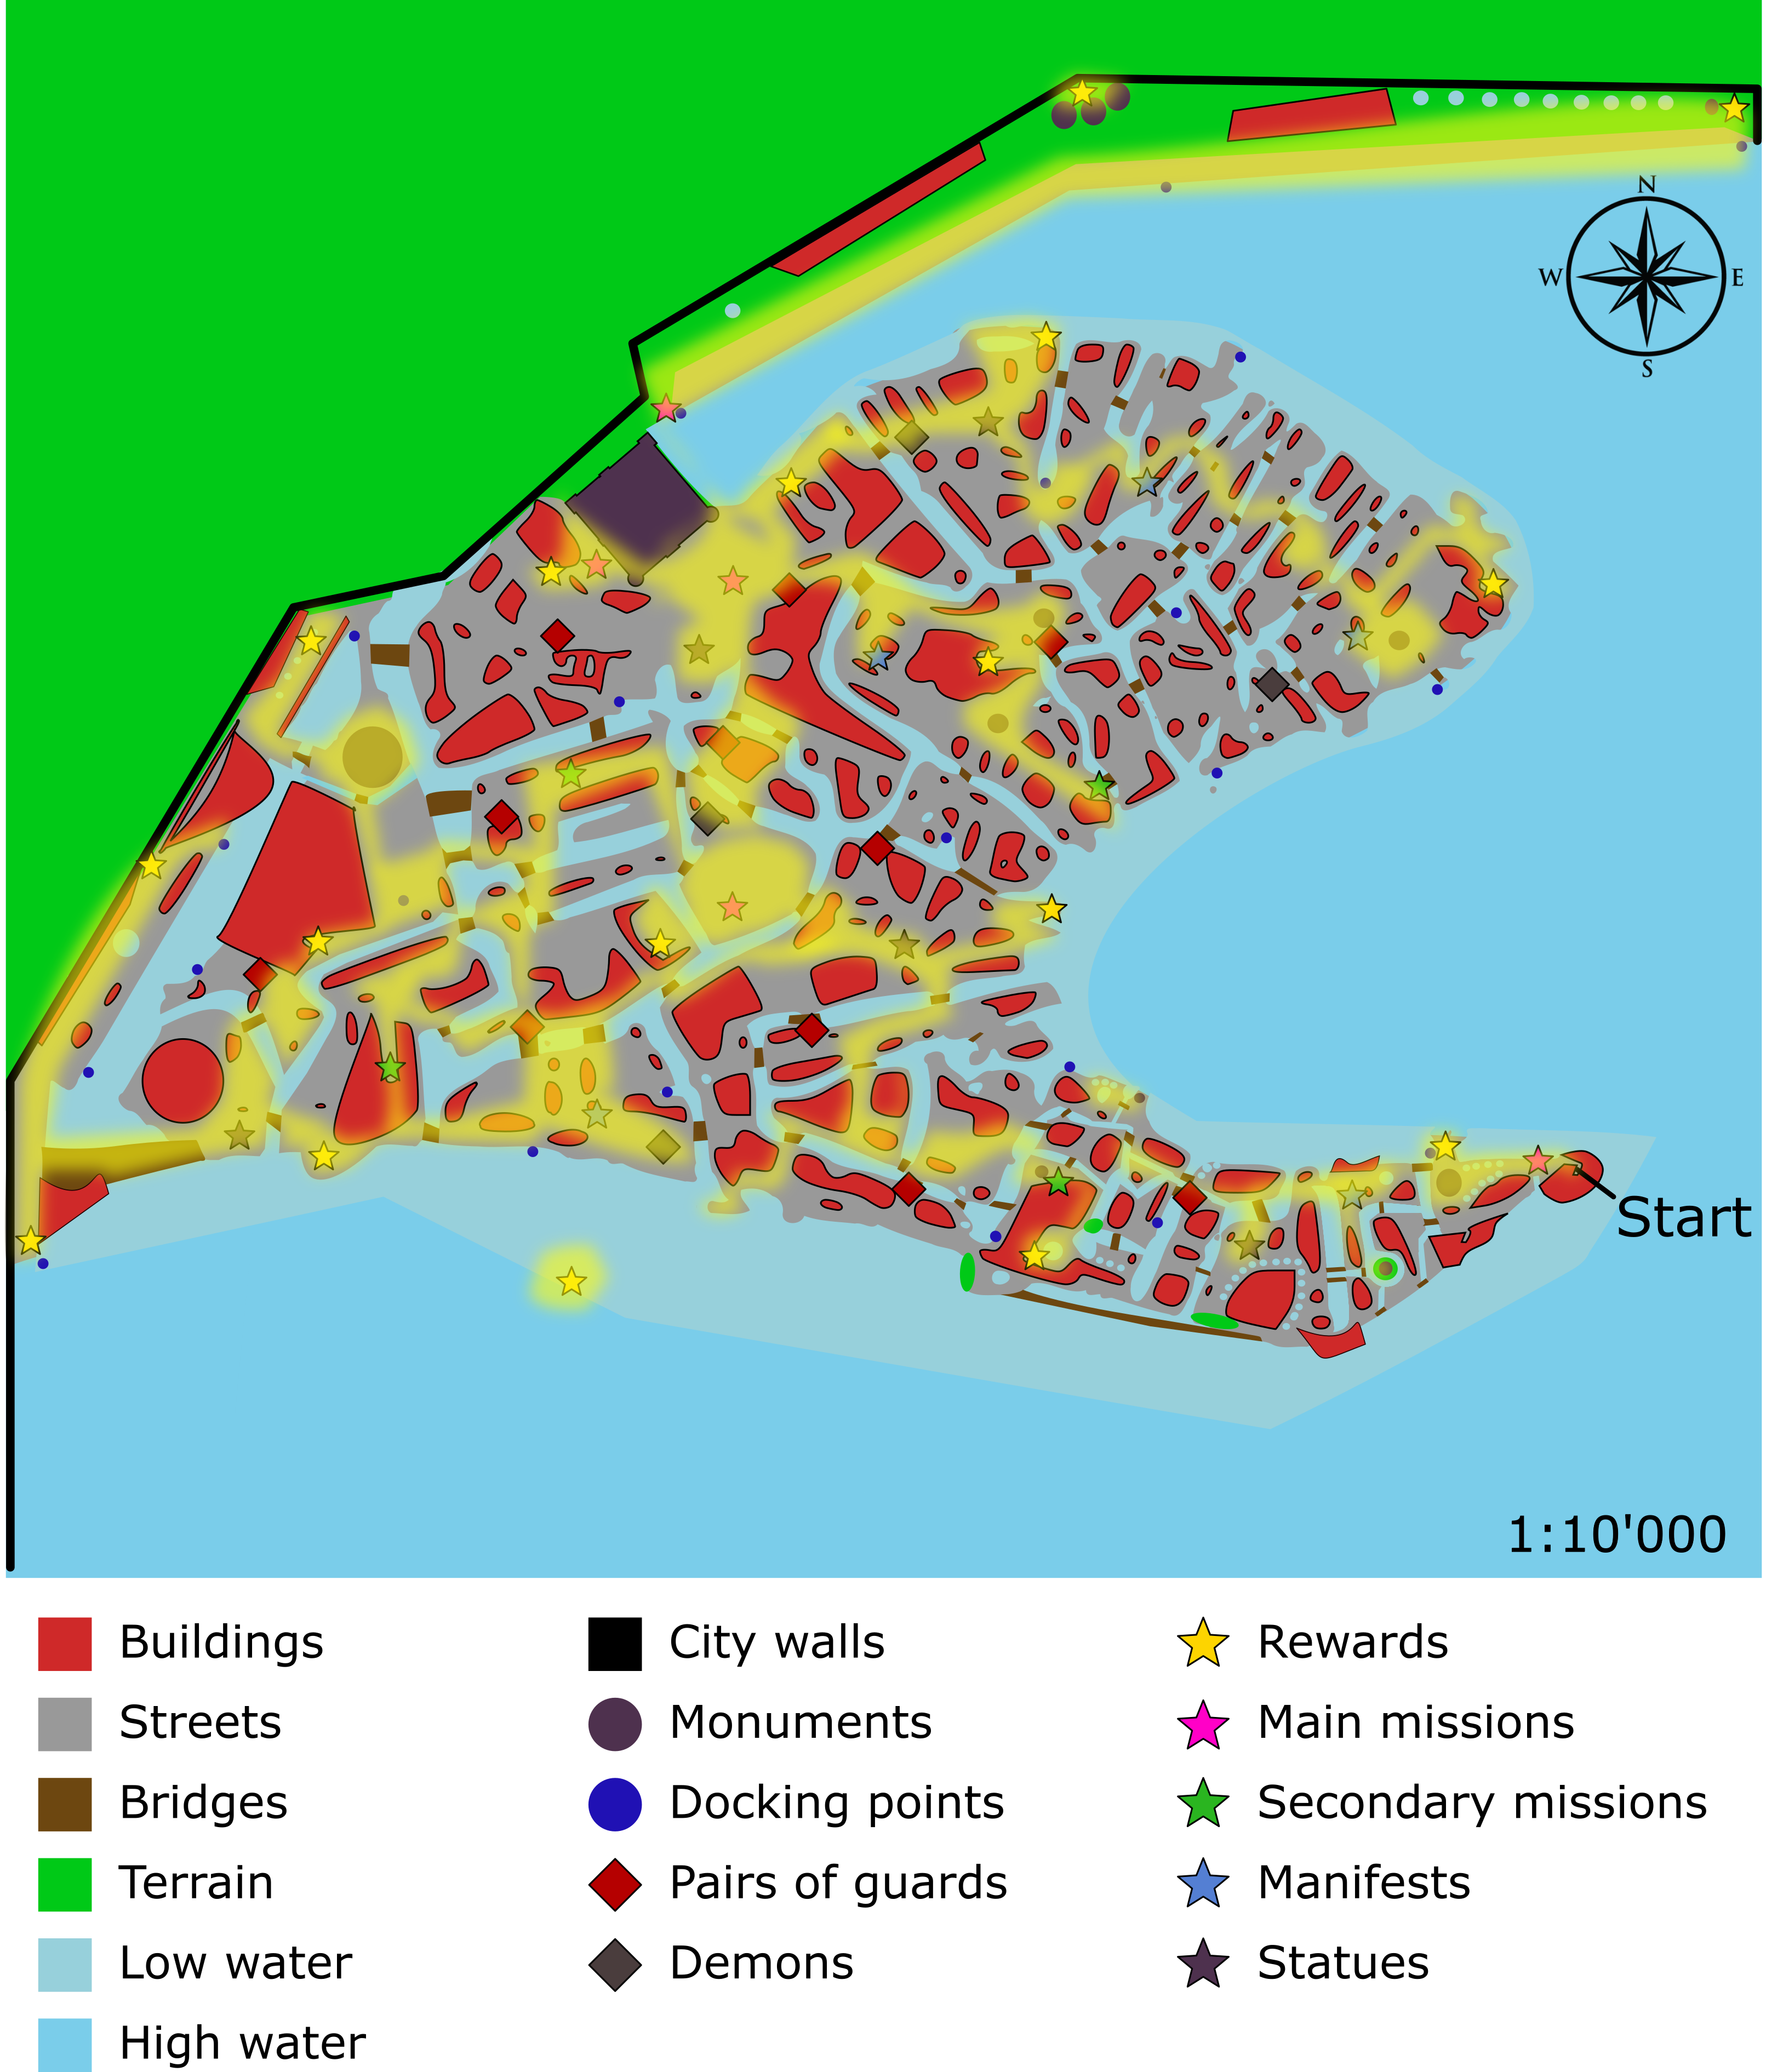
\includegraphics[width=\textwidth]{Images/Maps/dynamiaLighting}
  \caption{Lighting of Dynamia}
\end{figure}

\begin{figure}[H]
  \centering
  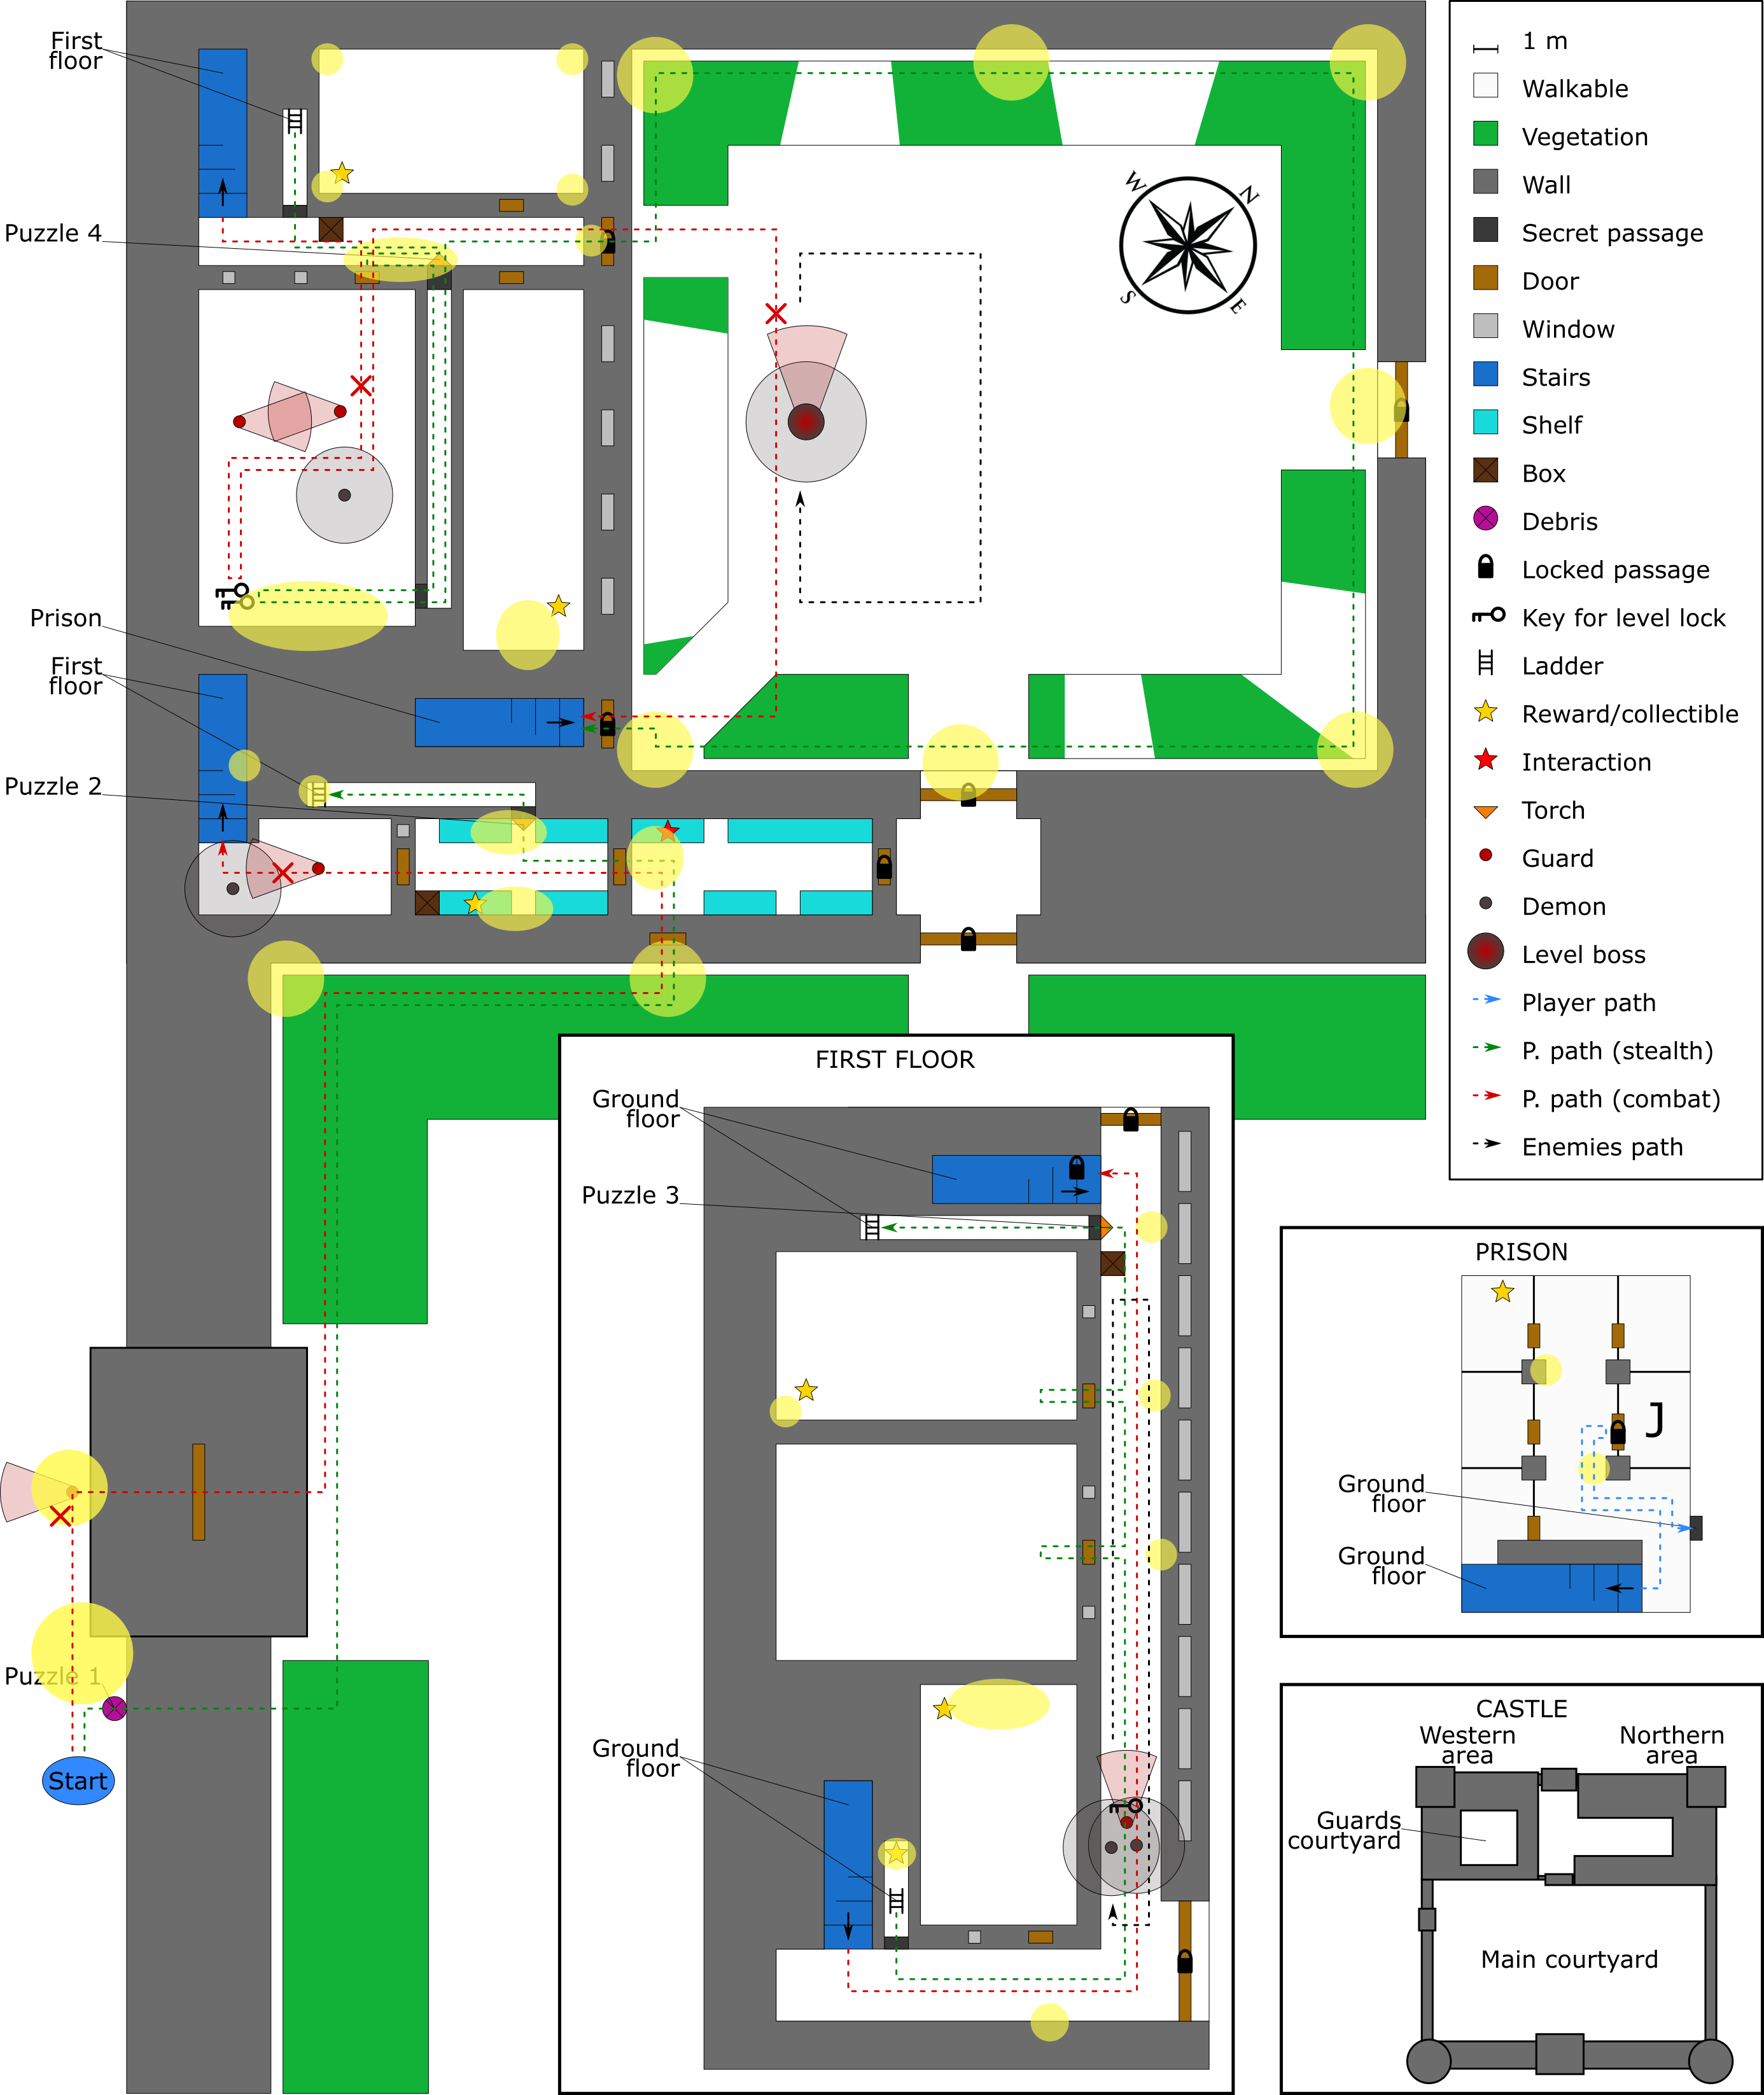
\includegraphics[width=\textwidth]{Images/Maps/castleOfDynamiaLighting}
  \caption{Lighting of the Castle of Dynamia}
\end{figure}

We have chosen to light some streets in the city and some spots in the castle in order to give to the player some clues about the optimal paths he can follow to both find rewards and make progresses in the main story, exploring meanwhile the whole map and seeing all of the peculiar assets that will be produced for the monuments and the landmarks.

In the city the illumination will be created with light poles, that will be some good reference points along with the torches in the castle in case the player gets lost or wants to get back on the optimal path and they will be also good hints to reveal the presence of rewards or some hidden elements.

\begin{figure}[H]
  \centering
  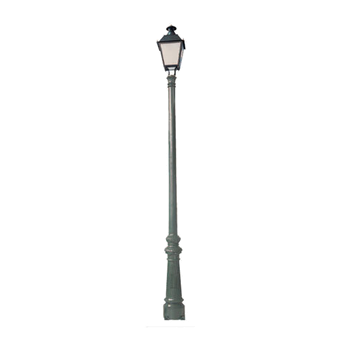
\includegraphics[height=12cm]{Images/Landmarks/lightPole}
  \caption{Reference images for the light poles in the city}
\end{figure}

\begin{figure}[H]
  \centering
  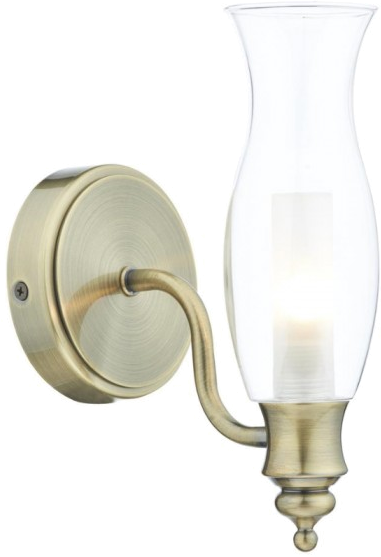
\includegraphics[height=12cm]{Images/Landmarks/gasLamp}
  \caption{Reference images for the gas lamps in the Castle}
\end{figure}

\begin{figure}[H]
  \centering
  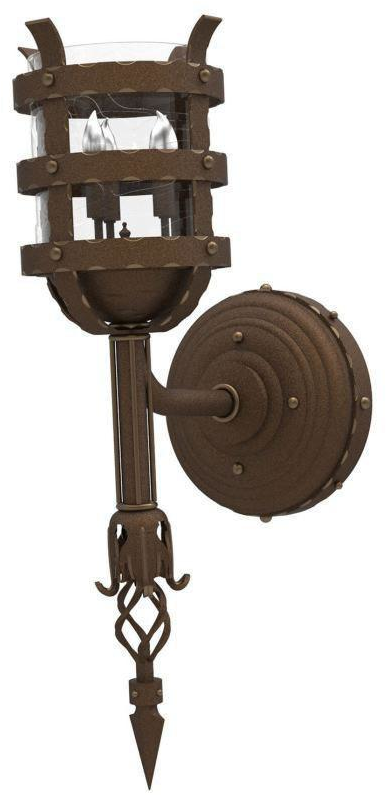
\includegraphics[height=12cm]{Images/Landmarks/torch}
  \caption{Reference images for the old torches in the Castle}
\end{figure}
